\documentclass[11pt,a4paper]{article}

% ============================================================
%                         PACKAGES
% ============================================================

\usepackage{amsmath,amssymb,mathtools}

\usepackage{tikz}
\usetikzlibrary{angles,quotes,calc,arrows.meta,intersections,positioning,decorations.pathreplacing}

\usepackage{geometry}
\usepackage{xcolor}
\usepackage{tcolorbox}
\usepackage{pagecolor}
\usepackage{fontspec}
\usepackage{microtype}
\usepackage{hyperref}

% ============================================================
%                         CONFIGURATION
% ============================================================

\geometry{
    top=2.2cm,
    bottom=2.2cm,
    left=2.3cm,
    right=2.3cm
}

% ============================================================
%                         COULEURS
% ============================================================

\definecolor{background}{HTML}{010402}
\definecolor{text}{HTML}{F0F0F0}
\definecolor{muted}{HTML}{999999}

\definecolor{accent}{HTML}{64B5F6}
\definecolor{accent2}{HTML}{BA68C8}
\definecolor{green}{HTML}{81C784}
\definecolor{orange}{HTML}{FFB74D}
\definecolor{red}{HTML}{E57373}

\definecolor{boxbg}{HTML}{050505}
\definecolor{grid}{HTML}{030303}

\pagecolor{background}
\color{text}

% ============================================================
%                         POLICE
% ============================================================

\setmainfont{Latin Modern Roman}

% ============================================================
%                         HYPERLIENS
% ============================================================

\hypersetup{
    colorlinks=true,
    linkcolor=accent,
    urlcolor=accent,
    citecolor=accent
}

% ============================================================
%                         COMMANDES
% ============================================================

\newcommand{\R}{\mathbb{R}}

\newcommand{\vect}[1]{
    \begin{pmatrix}
        #1
    \end{pmatrix}
}

% ============================================================
%                         BOXES
% ============================================================

\newtcolorbox{definitionbox}{
    colback=boxbg,
    colframe=accent!70!black,
    coltext=text,
    boxrule=0.7pt,
    arc=3mm,
    left=5mm,
    right=5mm,
    top=3mm,
    bottom=3mm
}

\newtcolorbox{importantbox}{
    colback=boxbg,
    colframe=orange!70!black,
    coltext=text,
    boxrule=0.7pt,
    arc=3mm,
    left=5mm,
    right=5mm,
    top=3mm,
    bottom=3mm
}

\newcommand{\sectiontitle}[1]{
    \section{#1}
}

% ============================================================
%                         STYLES TIKZ
% ============================================================

\tikzset{
    axis/.style={
        -{Latex[length=2.5mm]},
        line width=0.8pt,
        color=muted
    },
    vector/.style={
        -{Latex[length=2.5mm]},
        line width=1.3pt
    },
    construction/.style={
        dashed,
        line width=0.7pt,
        color=muted
    },
    pointlabel/.style={
        font=\small,
        inner sep=2pt
    },
    figurelabel/.style={
        font=\small
    }
}

% ============================================================
%                         DOCUMENT
% ============================================================

\begin{document}

% ============================================================
%                         PAGE DE GARDE
% ============================================================

\begin{center}

\vspace*{2.5cm}

{
\fontsize{38}{45}\selectfont\bfseries
Matrices
}

\vspace{0.4cm}

{
\fontsize{20}{25}\selectfont
Une construction géométrique en dimension 2
}

\vspace{1.2cm}

% ============================================================
% FIGURE DE GARDE
% ============================================================

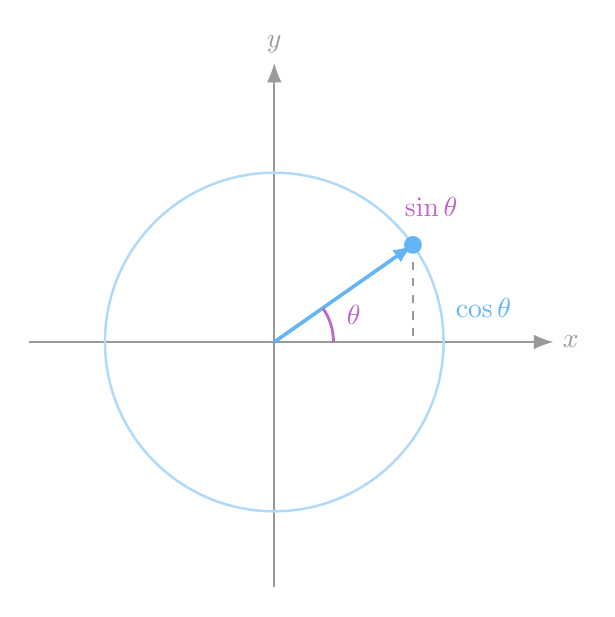
\begin{tikzpicture}[scale=2.15]

    % Axes
    \draw[axis]
        (-1.45,0) -- (1.65,0)
        node[right,inner sep=3pt] {$x$};

    \draw[axis]
        (0,-1.45) -- (0,1.65)
        node[above,inner sep=3pt] {$y$};

    % Cercle
    \draw[accent!50,line width=0.9pt]
        (0,0) circle (1);

    % Angle
    \def\a{35}

    % Rayon
    \draw[vector,accent]
        (0,0)
        -- ({cos(\a)},{sin(\a)});

    % Projection
    \draw[construction]
        ({cos(\a)},{sin(\a)})
        -- ({cos(\a)},0);

    % Point
    \fill[accent]
        ({cos(\a)},{sin(\a)})
        circle (1.5pt);

    % Angle
    \draw[accent2,line width=1pt]
        (0.35,0)
        arc (0:\a:0.35);

    \node[
        accent2,
        inner sep=2pt
    ]
        at (0.47,0.16)
        {$\theta$};

    % Labels
    \node[
        accent,
        anchor=west,
        inner sep=3pt
    ]
        at (1.02,0.20)
        {$\cos\theta$};

    \node[
        accent2,
        anchor=west,
        inner sep=3pt
    ]
        at (0.72,0.80)
        {$\sin\theta$};

\end{tikzpicture}

\vfill

{\color{muted}
De la trigonométrie aux transformations linéaires
}

\vspace{1cm}

\end{center}

\newpage

% ============================================================
%                         INTRODUCTION
% ============================================================

\sectiontitle{Introduction}

Ce document présente une construction progressive des matrices
dans un environnement à deux dimensions.

L'objectif n'est pas simplement de mémoriser des formules.
Nous allons essayer de comprendre \emph{pourquoi} ces formules
existent.

L'idée centrale est simple :

\begin{definitionbox}

Une matrice peut être interprétée comme une règle qui transforme
les coordonnées d'un vecteur.

\[
\boxed{
\text{vecteur}
\quad\xrightarrow{\text{matrice}}\quad
\text{vecteur transformé}
}
\]

\end{definitionbox}

Pour construire cette idée proprement, il faut d'abord comprendre
la géométrie des rotations.

Et pour comprendre les rotations, nous devons revenir à la
trigonométrie.

% ============================================================
%                         SECTION 1
% ============================================================

\sectiontitle{Le cercle trigonométrique}

Considérons le cercle unité :

\[
x^2+y^2=1.
\]

Un point du cercle peut être obtenu en partant de l'origine,
puis en parcourant une distance angulaire $\theta$.

% ============================================================
% FIGURE CERCLE UNITE
% ============================================================

\begin{center}

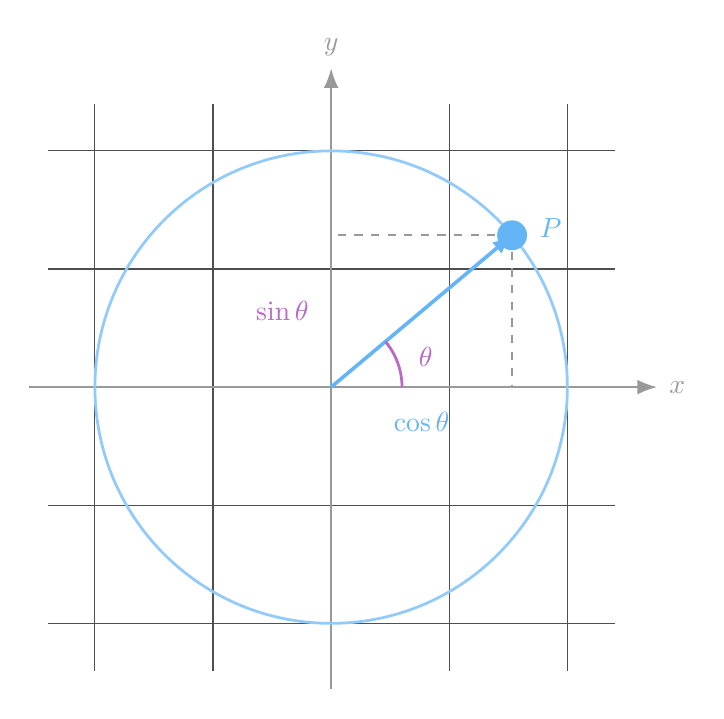
\begin{tikzpicture}[scale=3.0]

    \def\a{40}

    % Grille
    \draw[grid!70,step=0.5]
        (-1.2,-1.2) grid (1.2,1.2);

    % Axes
    \draw[axis]
        (-1.28,0) -- (1.38,0)
        node[right,inner sep=4pt] {$x$};

    \draw[axis]
        (0,-1.28) -- (0,1.35)
        node[above,inner sep=4pt] {$y$};

    % Cercle
    \draw[accent!70,line width=1pt]
        (0,0) circle (1);

    % Rayon
    \draw[vector,accent]
        (0,0)
        -- ({cos(\a)},{sin(\a)});

    % Projection horizontale
    \draw[construction]
        ({cos(\a)},{sin(\a)})
        -- ({cos(\a)},0);

    % Projection verticale
    \draw[construction]
        ({cos(\a)},{sin(\a)})
        -- (0,{sin(\a)});

    % Point
    \fill[accent]
        ({cos(\a)},{sin(\a)})
        circle (1.8pt);

    % Angle
    \draw[accent2,line width=1pt]
        (0.30,0)
        arc (0:\a:0.30);

    \node[
        accent2,
        inner sep=2pt
    ]
        at (0.40,0.13)
        {$\theta$};

    % cos theta
    \node[
        accent,
        anchor=north,
        inner sep=2pt
    ]
        at ({cos(\a)/2},-0.08)
        {$\cos\theta$};

    % sin theta
    \node[
        accent2,
        anchor=east,
        inner sep=2pt
    ]
        at (-0.07,{sin(\a)/2})
        {$\sin\theta$};

    % Point P
    \node[
        accent,
        anchor=west,
        inner sep=3pt
    ]
        at ({cos(\a)+0.08},{sin(\a)+0.03})
        {$P$};

\end{tikzpicture}

\end{center}

Comme le rayon du cercle vaut $1$, les coordonnées du point $P$
sont exactement :

\[
\boxed{
P=(\cos\theta,\sin\theta)
}
\]

Autrement dit,

\[
x=\cos\theta,
\qquad
y=\sin\theta.
\]

Cette représentation va devenir fondamentale.

% ============================================================
%                         SECTION 2
% ============================================================

\sectiontitle{Une première relation fondamentale}

Le point $P$ appartient au cercle unité.

Il vérifie donc :

\[
x^2+y^2=1.
\]

En remplaçant $x$ et $y$ par leurs expressions trigonométriques :

\[
\boxed{
\cos^2\theta+\sin^2\theta=1
}
\]

Cette identité vient directement de la géométrie du cercle.

% ============================================================
%                         SECTION 3
% ============================================================

\sectiontitle{Que se passe-t-il lorsqu'on additionne deux angles ?}

Considérons maintenant deux angles $a$ et $b$.

Nous voulons comprendre géométriquement ce que signifie :

\[
a+b.
\]

On peut interpréter cette somme comme deux rotations successives.

\[
\boxed{
\text{rotation de }a
\quad\longrightarrow\quad
\text{rotation de }b
\quad=\quad
\text{rotation de }(a+b)
}
\]

Pour trouver $\cos(a+b)$, nous allons regarder la projection
du vecteur obtenu après ces deux rotations.

% ============================================================
% FIGURE ADDITION DES ANGLES
% ============================================================

\begin{center}

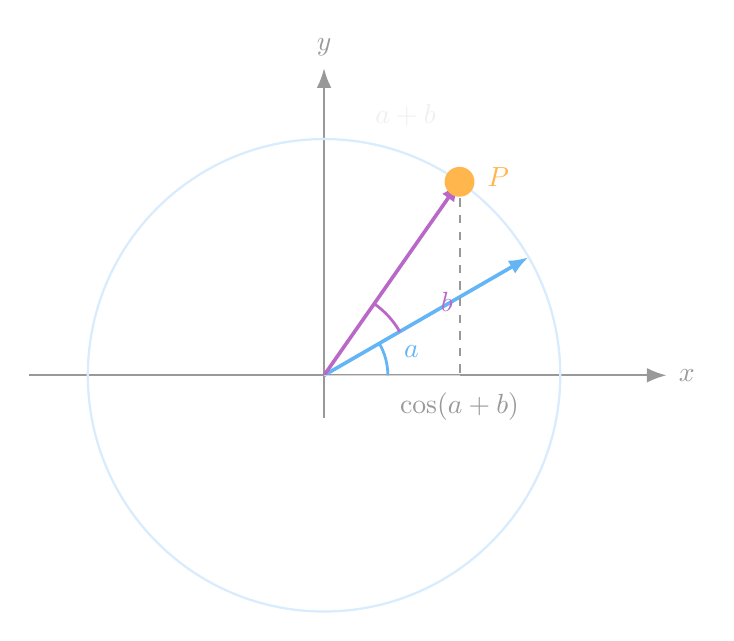
\begin{tikzpicture}[scale=3.0]

    \def\a{30}
    \def\b{25}

    % Coordonnées calculées
    \pgfmathsetmacro{\xa}{cos(\a)}
    \pgfmathsetmacro{\ya}{sin(\a)}
    \pgfmathsetmacro{\xf}{cos(\a+\b)}
    \pgfmathsetmacro{\yf}{sin(\a+\b)}

    % Axes
    \draw[axis]
        (-1.25,0) -- (1.45,0)
        node[right,inner sep=4pt] {$x$};

    \draw[axis]
        (0,-0.18) -- (0,1.30)
        node[above,inner sep=4pt] {$y$};

    % Cercle
    \draw[accent!25,line width=0.8pt]
        (0,0) circle (1);

    % Premier rayon
    \draw[vector,accent]
        (0,0) -- (\xa,\ya);

    % Rayon final
    \draw[vector,accent2]
        (0,0) -- (\xf,\yf);

    % Projection
    \draw[construction]
        (\xf,\yf) -- (\xf,0);

    % Projection horizontale
    \draw[muted!40]
        (0,0) -- (\xf,0);

    % Angle a
    \draw[accent,line width=1pt]
        (0.27,0)
        arc (0:\a:0.27);

    % Angle b
    \draw[accent2,line width=1pt]
        ({0.37*cos(\a)},{0.37*sin(\a)})
        arc (\a:{\a+\b}:0.37);

    % Label a
    \node[
        accent,
        inner sep=2pt
    ]
        at (0.37,0.10)
        {$a$};

    % Label b
    \node[
        accent2,
        inner sep=2pt
    ]
        at (0.52,0.31)
        {$b$};

    % Point final
    \fill[orange]
        (\xf,\yf)
        circle (1.8pt);

    % Label P
    \node[
        orange,
        anchor=west,
        inner sep=3pt
    ]
        at ({\xf+0.08},{\yf+0.02})
        {$P$};

    % Angle total
    \node[
        color=text,
        anchor=west,
        inner sep=3pt
    ]
    at (0.18,1.10)
    {$a+b$};

    % Projection
    \node[
        muted,
        anchor=north,
        inner sep=2pt
    ]
        at (\xf,-0.05)
        {$\cos(a+b)$};

\end{tikzpicture}

\end{center}

Pour aller plus loin, il est utile de décomposer le vecteur
final en deux directions.

La composante horizontale provient de deux contributions :

\[
\cos a\cos b
\]

et

\[
-\sin a\sin b.
\]

Ainsi :

\[
\boxed{
\cos(a+b)
=
\cos a\cos b-\sin a\sin b
}
\]

De même, pour la composante verticale :

\[
\boxed{
\sin(a+b)
=
\sin a\cos b+\cos a\sin b
}
\]

Ces deux identités sont exactement celles dont nous aurons besoin
pour construire les matrices de rotation.

% ============================================================
%                         SECTION 4
% ============================================================

\sectiontitle{Du cercle aux vecteurs}

Un vecteur du plan peut s'écrire :

\[
\vec v=
\begin{pmatrix}
x\\
y
\end{pmatrix}.
\]

Prenons le vecteur unitaire :

\[
\vec u=
\begin{pmatrix}
1\\
0
\end{pmatrix}.
\]

Après une rotation d'un angle $\theta$, ce vecteur devient :

\[
\vec u'=
\begin{pmatrix}
\cos\theta\\
\sin\theta
\end{pmatrix}.
\]

Mais que se passe-t-il pour le vecteur vertical

\[
\vec w=
\begin{pmatrix}
0\\
1
\end{pmatrix}?
\]

Une rotation de $\theta$ lui donne :

\[
\vec w'
=
\begin{pmatrix}
-\sin\theta\\
\cos\theta
\end{pmatrix}.
\]

Nous avons donc deux vecteurs :

\[
\begin{pmatrix}
1\\
0
\end{pmatrix}
\longrightarrow
\begin{pmatrix}
\cos\theta\\
\sin\theta
\end{pmatrix}
\]

et

\[
\begin{pmatrix}
0\\
1
\end{pmatrix}
\longrightarrow
\begin{pmatrix}
-\sin\theta\\
\cos\theta
\end{pmatrix}.
\]

Ces deux colonnes vont former notre matrice.

% ============================================================
%                         SECTION 5
% ============================================================

\sectiontitle{Construire la matrice de rotation}

On place les vecteurs transformés comme colonnes :

\[
\boxed{
R(\theta)=
\begin{pmatrix}
\cos\theta & -\sin\theta\\
\sin\theta & \cos\theta
\end{pmatrix}
}
\]

Cette matrice contient donc directement la géométrie de la rotation.

Appliquons-la à un vecteur :

\[
\begin{pmatrix}
x'\\
y'
\end{pmatrix}
=
\begin{pmatrix}
\cos\theta & -\sin\theta\\
\sin\theta & \cos\theta
\end{pmatrix}
\begin{pmatrix}
x\\
y
\end{pmatrix}.
\]

En effectuant le produit matriciel :

\[
\boxed{
x'=x\cos\theta-y\sin\theta
}
\]

et

\[
\boxed{
y'=x\sin\theta+y\cos\theta
}
\]

Voilà la transformation géométrique complète.

% ============================================================
% FIGURE ROTATION
% ============================================================

\begin{center}

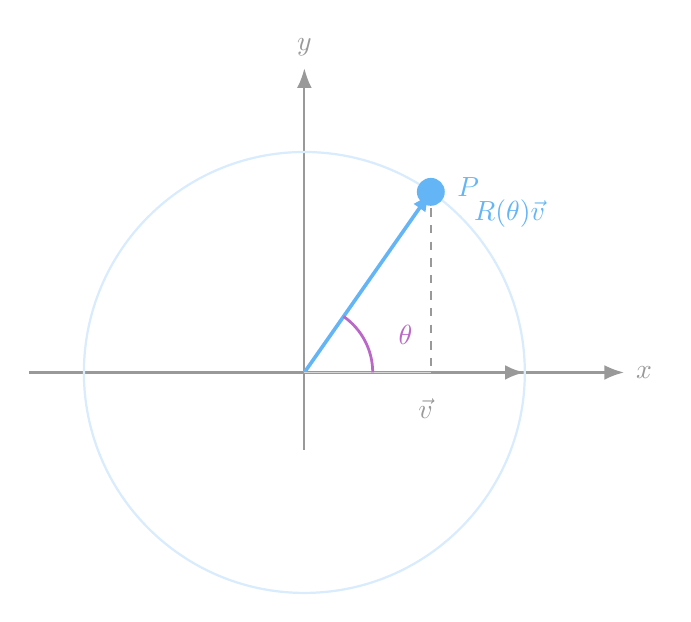
\begin{tikzpicture}[scale=2.8]

    \def\a{55}

    \pgfmathsetmacro{\xf}{cos(\a)}
    \pgfmathsetmacro{\yf}{sin(\a)}

    % Axes
    \draw[axis]
        (-1.25,0) -- (1.45,0)
        node[right,inner sep=4pt] {$x$};

    \draw[axis]
        (0,-0.35) -- (0,1.38)
        node[above,inner sep=4pt] {$y$};

    % Cercle
    \draw[accent!25,line width=0.8pt]
        (0,0) circle (1);

    % Vecteur initial
    \draw[vector,muted]
        (0,0) -- (1,0);

    % Vecteur final
    \draw[vector,accent]
        (0,0) -- (\xf,\yf);

    % Projection
    \draw[construction]
        (\xf,\yf) -- (\xf,0);

    % Projection horizontale
    \draw[muted!40]
        (0,0) -- (\xf,0);

    % Angle
    \draw[accent2,line width=1pt]
        (0.31,0)
        arc (0:\a:0.31);

    % theta
    \node[
        accent2,
        anchor=west,
        inner sep=2pt
    ]
        at (0.40,0.17)
        {$\theta$};

    % vecteur initial
    \node[
        muted,
        anchor=north,
        inner sep=3pt
    ]
        at (0.55,-0.08)
        {$\vec v$};

    % vecteur final
    \node[
        accent,
        anchor=west,
        inner sep=3pt
    ]
        at (0.73,0.72)
        {$R(\theta)\vec v$};

    % Point
    \fill[accent]
        (\xf,\yf)
        circle (1.8pt);

    % Label point
    \node[
        accent,
        anchor=west,
        inner sep=3pt
    ]
        at ({\xf+0.08},{\yf+0.02})
        {$P$};

\end{tikzpicture}

\end{center}

% ============================================================
%                         SECTION 6
% ============================================================

\sectiontitle{Pourquoi les matrices sont puissantes}

Une matrice n'est pas seulement un tableau de nombres.

Elle représente une transformation.

Par exemple :

\[
\begin{pmatrix}
2&0\\
0&1
\end{pmatrix}
\]

transforme :

\[
\begin{pmatrix}
x\\
y
\end{pmatrix}
\longrightarrow
\begin{pmatrix}
2x\\
y
\end{pmatrix}.
\]

Le plan est étiré horizontalement.

Une autre matrice :

\[
\begin{pmatrix}
1&0\\
0&2
\end{pmatrix}
\]

étire le plan verticalement.

Et notre matrice de rotation :

\[
\begin{pmatrix}
\cos\theta&-\sin\theta\\
\sin\theta&\cos\theta
\end{pmatrix}
\]

fait tourner les vecteurs.

% ============================================================
%                         SECTION 7
% ============================================================

\sectiontitle{Composer plusieurs transformations}

Supposons que nous effectuions une rotation d'un angle $a$,
puis une rotation d'un angle $b$.

Nous avons :

\[
R(a)R(b).
\]

Calculons :

\[
R(a)R(b)
=
\begin{pmatrix}
\cos a&-\sin a\\
\sin a&\cos a
\end{pmatrix}
\begin{pmatrix}
\cos b&-\sin b\\
\sin b&\cos b
\end{pmatrix}.
\]

Le produit donne :

\[
=
\begin{pmatrix}
\cos a\cos b-\sin a\sin b
&
-\cos a\sin b-\sin a\cos b
\\
\sin a\cos b+\cos a\sin b
&
-\sin a\sin b+\cos a\cos b
\end{pmatrix}.
\]

En utilisant les identités trigonométriques précédentes :

\[
\boxed{
R(a)R(b)=
\begin{pmatrix}
\cos(a+b)&-\sin(a+b)\\
\sin(a+b)&\cos(a+b)
\end{pmatrix}
}
\]

donc :

\[
\boxed{
R(a)R(b)=R(a+b)
}
\]

C'est une idée importante :

\begin{importantbox}

\[
\boxed{
\text{composer deux transformations}
\quad\Longleftrightarrow\quad
\text{multiplier leurs matrices}
}
\]

\end{importantbox}

La multiplication matricielle encode donc directement la composition
des transformations géométriques.

% ============================================================
%                         SECTION 8
% ============================================================

\sectiontitle{Vers les transformations générales}

La rotation n'est qu'un exemple.

Une matrice générale :

\[
A=
\begin{pmatrix}
a&b\\
c&d
\end{pmatrix}
\]

transforme :

\[
\begin{pmatrix}
x\\
y
\end{pmatrix}
\]

en :

\[
\begin{pmatrix}
x'\\
y'
\end{pmatrix}
=
A
\begin{pmatrix}
x\\
y
\end{pmatrix}.
\]

Ainsi :

\[
\boxed{
x'=ax+by
}
\]

et

\[
\boxed{
y'=cx+dy
}
\]

En changeant les quatre coefficients $a,b,c,d$,
on peut produire de nombreuses transformations :

\[
\text{rotation},
\qquad
\text{étirement},
\qquad
\text{compression},
\qquad
\text{cisaillement},
\qquad
\text{réflexion}.
\]

Les matrices deviennent alors une sorte de langage permettant
de décrire la géométrie algébriquement.

% ============================================================
%                         CONCLUSION
% ============================================================

\sectiontitle{Conclusion}

Nous sommes partis d'une figure géométrique très simple :
le cercle unité.

Nous avons obtenu :

\[
P=(\cos\theta,\sin\theta).
\]

Puis la géométrie nous a conduit aux identités :

\[
\cos(a+b)
=
\cos a\cos b-\sin a\sin b
\]

et

\[
\sin(a+b)
=
\sin a\cos b+\cos a\sin b.
\]

Ces relations nous ont ensuite permis de construire :

\[
\boxed{
R(\theta)=
\begin{pmatrix}
\cos\theta&-\sin\theta\\
\sin\theta&\cos\theta
\end{pmatrix}
}
\]

qui transforme les vecteurs du plan par rotation.

Ainsi, une matrice peut être comprise non comme un simple tableau
de nombres, mais comme une représentation algébrique d'une
transformation géométrique.

\begin{center}

\vspace{1cm}

{\Large\color{accent}
Géométrie $\rightarrow$ vecteurs $\rightarrow$ matrices
}

\vspace{0.4cm}

{\color{muted}
Une même idée, exprimée dans différents langages.
}

\end{center}

\end{document}